
\documentclass[12pt]{iopart}
\newcommand{\gguide}{{\it Preparing graphics for IOP Publishing journals}}
%Uncomment next line if AMS fonts required
\usepackage{iopams}  
\usepackage{braket}
\usepackage{graphicx}
\usepackage{subfigure}
\usepackage{cite}

\begin{document}

\title[]{Observation of S-wave scattering of fermions accross a Feshbach resonance}

\author{D Genkina$^1$, LM Aycock$^{1,2}$, BK Stuhl$^1$, Hsin-I Lu$^1$ and IB Spielman
$^1$\footnote{Corresponding author}}

\address{$^1$Joint Quantum Institute, National Institute of Standards and Technology, and University of Maryland, Gaithersburg, MD, 20899 USA}
\address{$^2$Physics Department, Cornell University, Ithaca, NY 14850 USA}

\ead{spielman@umd.edu}

\begin{abstract}
We present results on mapping out an s-wave Feshbach resonance in fermionic $^{40}$K by directly observing atom scattering over a range of 
magnetic field strenghts. To optimize signal to noise, we develop techniques to interpret absorption imaging in the regime where recoil induced 
detuning corrections are significant. We apply these techniques to our s-wave scattering data to extract an estimate for the resonant magnetic
field value. These techniques can be applied to observation of effective p-wave scattering in the presence of spin-orbit coupling in a spin polarized 
Fermi gas.
\end{abstract}

\vspace{2pc}
\noindent{\it Keywords}: Quantum gases, Atomic physics, Something else

\maketitle

\section{Introduction}
Feshbach resonances are a staple tool in the study of cold Fermi gases. Interatomic interactions in Bose-Einstein condensates are easily detected due to the high density of the cloud. However, the density of Fermi clouds is reduced by a factor of $~10^3$ from that of BECs. This makes it necessary to enhance the scattering cross section to observe any effects of interaction. Feshbach resonances allow one to tune the scattering length by changing the magnetic field. Not ony do they enable detection of interactions, but they make it possible to tune interactions from attractive to repulsive, allowing for the phase transition from the BCS to BEC regime at sufficiently low temperatures. 
\par However, to take advantage of Feshbach resonances as a tool it  is first necessary to have a good undestanding of the relationship between the bias magnetic field and the scattering cross section near a Feshbach resonance for specific species and hyperfine states.  The exact value of the resonance is difficult to calculate analytically and must be determined experimentally. Currently, Feshbach resonances are mapped out by observing loss due to three-body inelastic scattering or by re-thermalization or anisotropic expansion measurements that infer the elastic scattering cross section from collective behavior of the cloud. 
\par We collide two clouds of $^{40}K$ atoms in a mixture of $\ket{9/2,-9/2}$ and $\ket{9/2,-7/2}$ hyperfine states and directly image the resulting s-wave scattering halo as a function magnetic field strength. This allows us to directly observe the enhancement in scattering without relying on collective behavior. However, even when the scattering is enhanced by the Feshbach resonance, the Fermi cloud is dilute enought that the number of scattered attoms is still very low compared to the number of atoms that pass through the other cloud unscattered. This poses a challenge for imaging both high and low atom numbers in the same shot.
\par In order to optimize the signal to noise for low atom numbers, we increased our imaging time.  However, above saturation absorption imaging at sufficiently long exposure times poses a particular problem - if the atoms have had time to absorb enough photons such that the recoil velocity Doppler shifts them from resonance on the order of the linewidth of the resonance, this recoil-induced detuning is a significant correction to the observed absorption of the probe light. In order to take this correction into account, we simulate the imaging process and use the results to extract the atom number and the scattered fraction from our images.
\par This paper is in two parts. In the first, we study absorption imaging in the presence of significant recoil-induced detuning and show how we use our results to interpret data. In the second, we describe our s-wave scattering experiment and, after correcting our data for recoil-induced detuning, extract a measure of the location of the Feshbach resonance in $^{40}K$. 

\section{Absorption imaging in the presence of strong recoil induced detuning}
Absorption imagaing is one of the two most common imaging techniques used in ultracold atomic physics, fluorescence imaging being the other. To obtain an absorption image, one shines an on or near resonant probe beam onto the atomic cloud, and captures the part of the beam that made it through the cloud onto a camera. Then, the atoms are allowed to leave the trap, and the probe light is shined directly at the camera, to calibrate the intensity of light that the atoms saw. The intensity in the second camera image at some point in time is called the initial intensity, $I_{0}(t)$, as it is assumed to be the intensity before interaction with atoms. The intensity in the first image at some point in time is called the final intensity, $I_f(t)$.  
\par It is convenient to define the optical density, $\nu=-\ln{\frac{\int{I_f(x,y,t)}\mathrm{d}t}{\int{I_0(x,y,t)}\mathrm{d}t}}$. Assuming the intensity seen by the camera during the first and second pulse is constant in time, this reduces to $\nu=-\ln{\frac{I_f(x,y)}{I_0(x,y)}}$. This is an observed quantity, and it is then the job of the experimentalist to relate it to the number of atoms $n = \int \rho\left(x,y,z\right) \,\mathrm{d}z$, where $\rho$ is the 3d atomic distribution, and $z$ is the imaging axis. Another useful quantity is the optical depth, $OD=\sigma_0\rho$, where $\sigma_0$ is the on-resonant scattering cross section. Though in general one needs a theoretical model to relate the optical density $\nu$ to the optical depth  and thus the atom number, it is convenient that in the limit of zero probe intensity, these quantities coincide, $OD_0=\nu$, as will be seen below. We call this $OD_0$, becaue it is the simplest, in a sense "0th order" model for relating the optical density to the optical depth.
\par The intensity of light from the beam as a function of distance is equal to the power scattered by the atoms. Without taking the atomic recoil velocity into account, and thus assuming both the intensity at every point in the cloud to be constant in time, this is given by \cite{Reinaudi07}
\begin{equation}
\frac{dI(z)}{dz}=-\rho\sigma_0\frac{I(z)}{1+I(z)/I_{sat}},
\end{equation}
 where  $I_{sat}$ is the saturation intensity. We've suppressed the x and y dependence, or alternatively we've focused on a single pixel.  This equation can be easily integrated over $z$ to obtain
\begin{equation} 
OD_1 =\sigma_0 n = \nu + \frac{I_0-I_f}{I_{sat}},
\label{eq2}
\end{equation}
 This gives us a model for the optical depth that includes a correction due to saturation intensity. In the limit of far below saturation probe intensity, it reduces to our "0th order" model, $OD_0$. 
\par Once you include the recoil velocity, the atoms become doppler shifted out of resonance and thus change the amount of proble light that will get absorbed. This detuning varies both with imaging time $t$ and distance along the propagation direction $z$ (Figure \ref{fig:detunedBlobs}). Thus, the intensity lost to the atoms also acquires a time dependence: 
\begin{equation}
\frac{dI(t,z)}{dz}=\sigma_0 \rho \frac{I(t,z)}{1+\frac{4}{\Gamma^2}\delta(t,z)^2 +I(t,z)/I_{sat}}, \label{eq3}
\end{equation}
where $\Gamma$ is the linewidth of the atomic transition, and $\delta$ is the detuning, given by 
\begin{equation}
\delta(t,z)=\frac{v_r}{\hbar c \rho}\int_0^t \frac{dI(z,\tau)}{dz}\,\mathrm{d}\tau, \label{eq4} 
\end{equation}
where  $v_r$ is the recoil velocity. In this case, one can no longer obtain a straightforward relation between the atom number and the intensities in the two absorption images.
\begin{figure}
	\includegraphics*[scale=0.57]{figure1}
\caption{Distribution of generalized detuning $\Delta=\frac{2\delta}{\Gamma}$ accross an atomic cloud of $^{40}K$ for three different imaging times, as obtained by numerical simulation.}  
\label{fig:detunedBlobs}
\end{figure}
\par One can consider this equation perturbatively in time and obtain corrections to second order in imaging time, $OD_2$  \cite{LJLthesis}. However, the perturbative treatment breaks down after about a recoil of imaging time (Figure \ref{fig:ODcorrections}). In order to adequately correct for the recoil induced detuning of the atoms, we must simulate the process and obtain numerical predictions for $I_f$ given a certain imaging time, atomic density, and probe intensity. 
\begin{figure}
	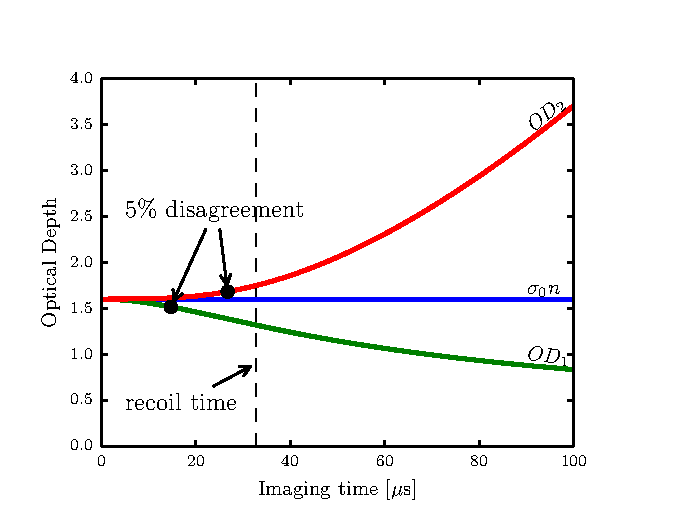
\includegraphics[scale=0.57]{figure2}
\caption{Using time dependent $I_f$ values obtained from recoil detuning corrected simulation of on-resonant imaging of $^{40}K$ atoms, this graph shows the optical depths each model would deduce from such images. The true optical depth is given at 1.6.$OD_1$ is the high probe intensity corrected optical depth given by \ref{eq2}. $OD_2$ is the model that includes high probe intensity corrections and imaging time corrections from expanding \ref{eq3},\ref{eq4} to second order in imaging time \cite{LJLthesis}. Note that the value obtained using the second order expansion in time starts to differ significantly from the true value after about 20us. The probe intensity is $0.8\, I_{sat}$. }  
\label{fig:ODcorrections}
\end{figure}
\par In the following, we describe two versions of this simulation. First, we take the simplistic approach that the on-axis distibution of atoms does not change dramatically durning the imaging time and can be treated statically. We test this approach in known limits and then use then check the validity of the static assumption. It turns out that, for realistic input parameters, this assumption is grossly incorrect. So, we take a slightly more sophisticated approach and allow the atoms to move within the cloud during the imaging time. This allows us to simulate the phase space evolution of atoms subjected to probe light. However,   
in the end we find that numerical differences in predicted OD only vary on the 0.05$\%$ level between the two models. 


\subsection{Stationary atom model}
In order to solve eq \ref{eq3},\ref{eq4}, we start with an input 1-d distribution of atom densities $\rho(z)$, usually gaussian in shape. We divide the cloud into spatial bins (the bin size was chosen such that decreasing the bin size further produced less than a 0.001$\%$ difference in the result).   Each bin carries a certain number of atoms. In this approximation, we keep the number of atoms in each bin constant. Then, we input a probe intensity, and propagate the intensity bin by bin according to \ref{eq3}, such that each bin only sees the probe intensity that was not absorbed in the previous bins. Then, we update the average velocity of the atoms in each bin according to \ref{eq4} for our time step size $dt$.  Then, we propagate the probe intensity through each bin again, starting with the same intensity at the first bin but this time taking into account the average recoil induced detuning of each bin in calculating the intensity aborbed. We continue this two-step process until we reach the desired imaging time.
\par We sum the intensity that made it through the entire cloud at each time step $\int_{t=0}^{t_f} I_f (\tau)\,\mathrm{d}\tau$, the observable that is actually detected on the first absorption image.  From this we can obtain a simulated optical density, $\nu _s = -\ln{\frac{\int I_f (\tau)\,\mathrm{d}\tau}{I_0 t_f}}$. This optical density depends on the initial probe intensity and the intput atom number, or optical depth. Thus, we can take our two absorption images, which give us a value for the optical density as well as $I_0$, and infer what optical depth would have to be put into the simulation to obtain the observed optical density. We call this inferred optical depth $OD_{corr}$, the optical depth corrected for recoil induced detuning effects.  
\par To check the validity of our simulation, we can take it to certain limits in which the probelm becomes analytically solvabale. In the limit that the probe intensity is much weaker than saturation, $I_0\ll I_{sat}$, the atoms will not absorb enough light to significantly detune from resonance. We can then neglect time dependence and \ref{eq3} reduces to 
\begin{equation}
\frac{dI(z)}{dz}=-\rho\sigma_0 I(z),
\end{equation}
from which we recover the simple
\begin{equation}
\sigma_0 n = OD_0 = \nu. \label{eq6}
\end{equation}
In the limit that the probe intensity is much stronger than saturation, $I_0\gg I_sat$, even far detuned atoms will absorb light at their maximum, allowing us to again neglect the time dependence and reduce \ref{eq3} to 
\begin{equation}
\frac{dI(z)}{dz}=-\rho\sigma_0 I_{sat}, 
\end{equation}
which integrates out to 
\begin{equation}
\sigma_0 n = \frac{I_0 - I_f}{I_{sat}}. \label{eq8}
\end{equation}
We recognize \ref{eq6} and \ref{eq8} as the two terms in the expression for $OD_1$, \ref{eq2}. Thus, in both limits $OD_{corr}$ should coincide with $OD_1$. Or equivalently, if the optical depth is an input parameter, in those limits both \ref{eq2} and our simulation should produce the same prediction for optical density. Indeed, they coincide as seen in figure \ref{fig:IsatLimits}.
\begin{figure}
	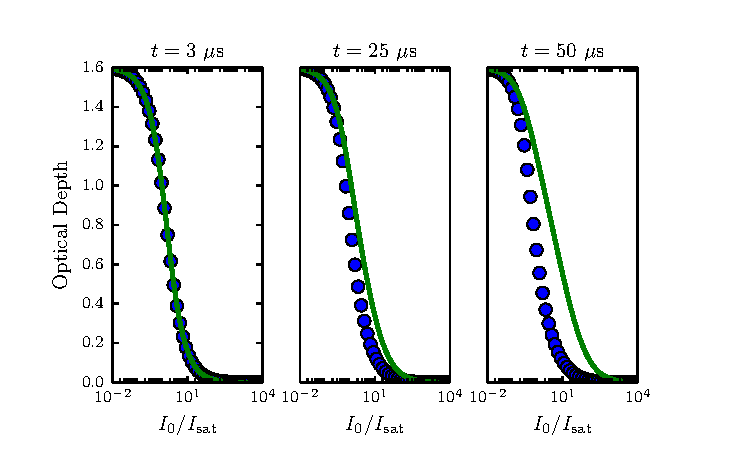
\includegraphics[scale=0.57]{figure3}
\caption{Optical densities as a function of probe intensity as predicted by the simulation and by \ref{eq2}, for three different imaging times. The predictions agree in both the high and low intensity limits, and differ for probe intensitites comparable to the saturation intensity. The difference is enhanced with increased imaging time.}  
\label{fig:IsatLimits}
\end{figure}
\par Encouraged by the reasonable behavior of our simulation, we can now use it to see if the stationary atom assumption is self consistent, ie if the distance travelled by the atoms in one bin during the imaging time is less than the bin size. However, as can be seen from figure \ref{fig:atomTravel}, it turns out that not only do the atoms travel more than the bin size, but they also travel more than the size of the whole cloud, and the back of the cloud travels less than the beginning for long enough imaging times. Thus, the atomic distribution as a function of position changes dramatically during the imaging time, and our stationary assumption is completely invalid. 
\begin{figure}
	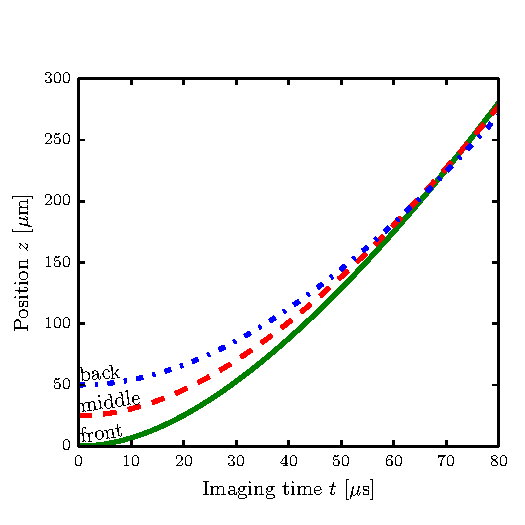
\includegraphics[scale=0.57]{figure4}
\caption{Position of atoms as a function of imaging time for atoms in the first, middle, and last bins of the simulation. The probe intensity here is $1.2 I_{sat}$, and the optical depth is 1.6.}  
\label{fig:atomTravel}
\end{figure}

\subsection{Traveling atom model}
To account for the changing atomic distribution during the imaging pulse, we shift our framework slightly from spatial bins of equal size with varying atoms number to superatoms. That is, we divide the initial atomic distribution into clumps of a set number of atoms, called superatoms, with initial positions that reflect the atomic distribution. The simulation then proceeds as before, propagating the probe light through one superatom at a time. But now, after the probe has been propagated through and the velocities of the superatoms are updated, the positions of the superatoms are advanced accordingly before the next time step is taken. Thus, we can simulate an evolving atomic distribution and track the resultant detunings. 
\par First, we should check the velocity behavior of our superatoms against calculable limits. One such limit is that of a single supeatom. In this case, the intensity seen by the superatom is constant at the full probe intensity, and the only time dependance in the problem is in the velocity, and thus detuning, of the superatom. \ref{eq4} can then be re-written as
\begin{equation}
\frac{d\delta\left(t\right)}{dt}=\frac{v_r}{\hbar c \rho}\frac{dI}{dz}\left(t\right)=\frac{v_r \sigma_0}{\hbar c}\frac{I_0}{1+\frac{4}{\Gamma^2}\delta(t)^2 +I_0/I_{sat}},
\label{eq9}
\end{equation} 
or in dimensionless form,
\begin{equation}
\frac{d\Delta(t)}{dt}= k v_r \frac{\tilde{I}}{1+\Delta^2+\tilde{I}},
\label{eq10}
\end{equation}
where $\Delta = 2\delta/\Gamma$, $\tilde{I} = I_0/I_{sat}$ and $k$ is the photonic wavevector. \ref{eq10} can be integrated and solved exactly with one real root. We can compare that result to our simulation, and it agrees as seen in figure \ref{fig:oneAtomVel}.
\begin{figure}
	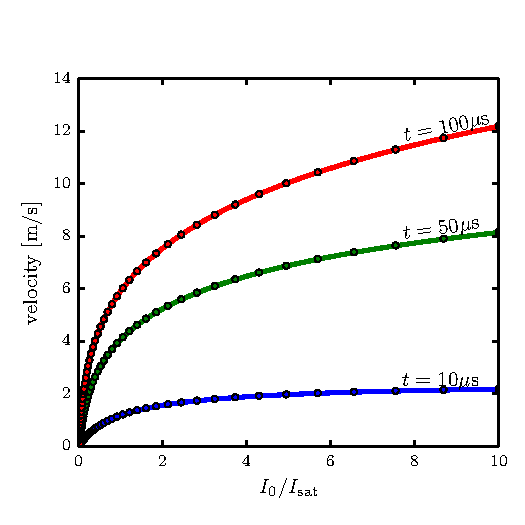
\includegraphics[scale=0.57]{figure5}
\caption{The velocity of a single superatom as a function of probe intensity for various imaging times. The dots represent simulation data, while the lines represent analytical solutions.}  
\label{fig:oneAtomVel}
\end{figure}
\par We are now in a position to study the time dependance of the cloud evolution. This can be visualized as a phase space evolution of superatoms, as seen in figure \ref{fig:phaseSpace}. We see that the cloud shape is actually strongly distorted in the imaging time. 
\begin{figure}
	\subfigure[]{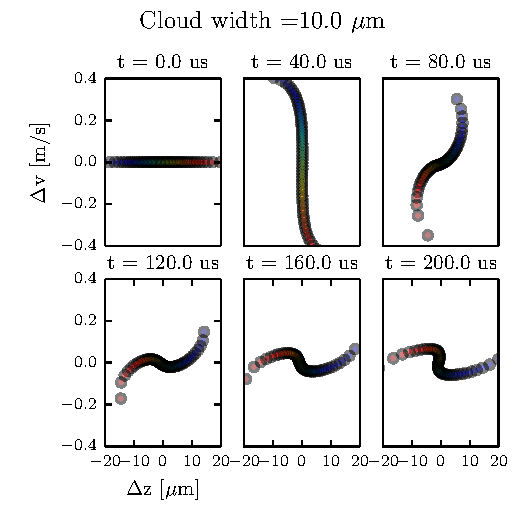
\includegraphics[scale=0.42]{figure6a}}
	\subfigure[]{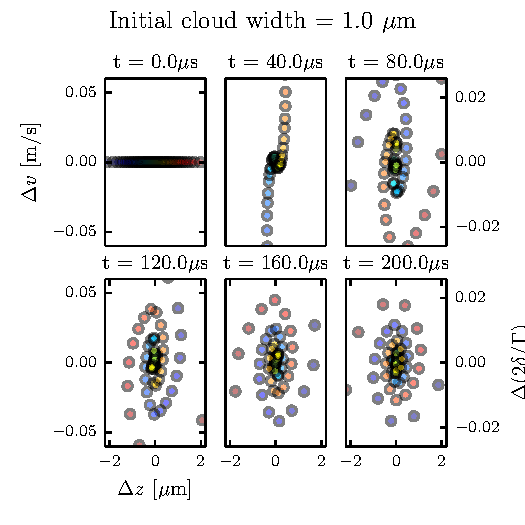
\includegraphics[scale=0.42]{figure6b}}
\caption{Phase space evolution of an atomic cloud exposed to probe light of $1.2 I_{sat}$. The optical depth is 1.6, and the initial cloud is a gaussian with width a. 10$\mu m$ and b. 1$\mu m$}  
\label{fig:phaseSpace}
\end{figure}
\par Having performed both the stationary and traveling atom simulations, we can compare the optical densities predicted by each, which we call $\nu_{corr1}$ and $\nu_{corr2}$ respectively. We find that, depite the significant changes in atomic distribution during the imaging time, the predicted optical densities are so slightly changed by including this effect that it is practically undetectable. In fact, the difference $\left|\nu_{corr1}-\nu_{corr2}\right|/\nu_{corr1} \le 0.05$. Thus, for the purposes of deducing the optical density from experimental optical depths, simply using a stationary model is sufficient. Furthermore, the actual atomic distribution $\rho(z)$ is largely irrelevant, and the only observable is the total atom number $n=\int\rho(z)\mathrm{d}z$. 
\begin{figure}
	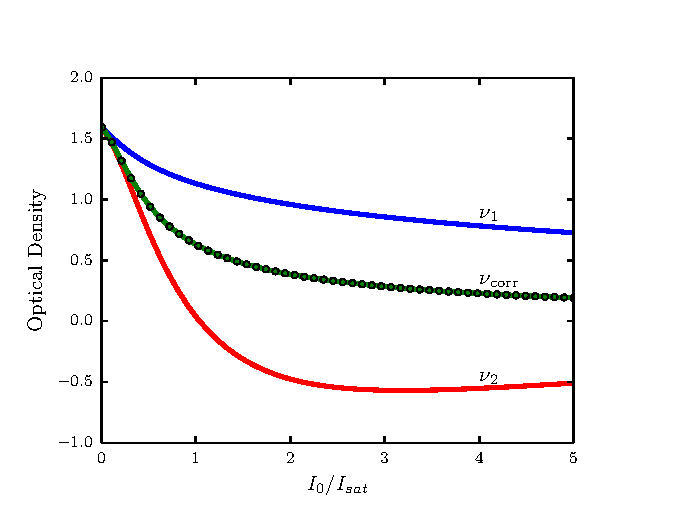
\includegraphics[scale=0.57]{figure7}
\caption{Predictions for optical density as a function of probe intensity for an imaging time $t=50\mu s$. Note that the two versions of simulated optical density, $\nu_{corr1}$ and $\nu_{corr2}$ are virtually indistinguishable. }  
\label{fig:atomTravel}
\end{figure}
\subsection{Calibration of saturation intensity}
Now we come to the question of how to interpret the actual ouput of an imaging camera. Each camera pixel outputs an integer number of "counts", proportional to the total energy it absobed during a pulse. The precise proportionality constant of these counts to the intensity as seen by the atoms depends on many factors, such as the quantum efficiency of the camera, the photoelectric conversion factor of the camera, and the polarization of the probe light. 
\par The most accurate way to determine this factor is through a direct experiment. In the limit where the system is adequately described by \ref{eq6}, only the ratio of the initial and final intensities matters, and thus this proportionality constant is irrelevant. In all other regimes, however, the ratio of the initial and final intensities to the saturation intensity also comes into play, making the proportionality constant significant. One way to approach this is to calibrate the saturation intensity in terms of camera counts per unit time. 
\par In order to calibrate the saturation intensity in camera counts per unit time, we take absorption images of a cloud of $^{40}K$ atoms at three different imaging times, 40us, 100us, and 200us, and at varying probe intensities. We pick a small square in the center of the cloud, where the atomic density is approximately uniform, and average the initial and final intensities of each pixel in the square. Thus, for each image we obtain one $I_0$ and one $I_f$, in units of counts per microsecond, or equavalently one optical density and one $I_0/I_{sat}$. We then do a least squares fit of $\nu_{corr}$, our simulated optical density, to the data. The two fit parameters are the optical depth at the center of the cloud, representing the actual atom number, and the value of $I_{sat}$ in counts per microsecond. As seen in figure \ref{fig:isatCalib}, the model produces a good fit to the experimental data. 
\begin{figure}
	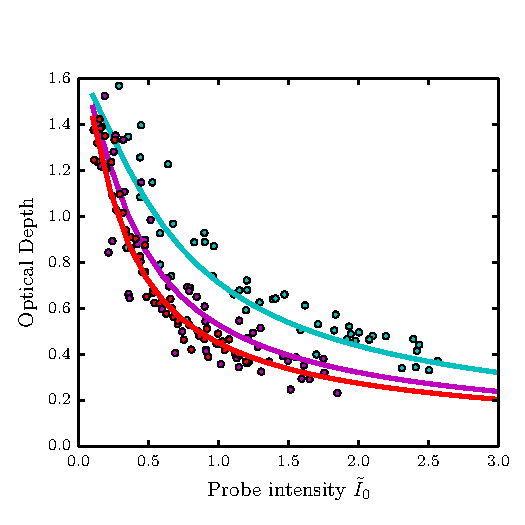
\includegraphics[scale=0.57]{figure8}
\caption{The optical density as a function of probe intensity for three imaging times. The dots represent experimental data and the lines represent the best fit of simulated data. The optimal fit parameters pictured are optical depth of 1.62 and saturation intensity of 29 counts/us. }  
\label{fig:isatCalib}
\end{figure}
\subsection{Signal to noise optimization}
\begin{figure}
	\subfigure[]{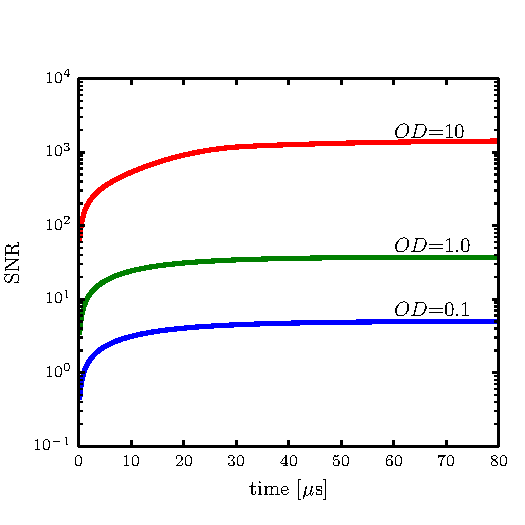
\includegraphics[scale=0.45]{figure9a}}
	\subfigure[]{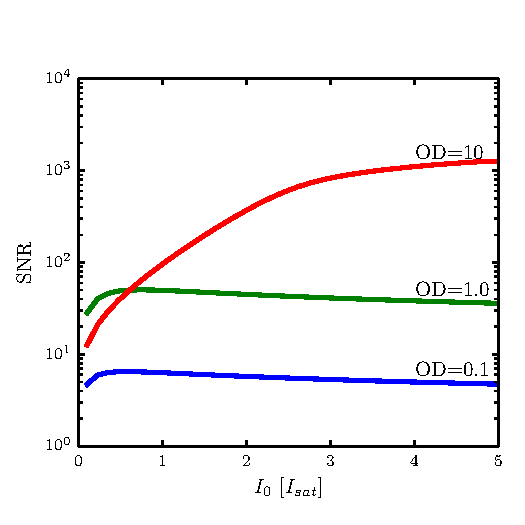
\includegraphics[scale=0.45]{figure9b}}
\caption{Dependance of detection uncertainty of optical depth on imaging time, after correcting for recoil induced detuning. a. Uncertainty at fixed probe intensity $I_0/I_{sat}=2.6$ for a range of optical depths and b. fixed $OD=1.5$ for a range of probe intensities.}  
\label{fig:SNR}
\end{figure}
\section{S-wave scattering experiment}
\subsection{Experimental setup}
\subsection{Methods}
\subsection{Results}
\section{Conclusion}
\bibliography{refs}{}
\bibliographystyle{plain}

\end{document}

